\section{Auswertung}
\label{sec:Auswertung}

\subsection{Fourier-Analyse}
\label{sec:Analyse}
In der folgenden Messreihe werden drei periodische elektrische Schwingungen in ihre Fourier-Komponenten zerlegt und diese mit den Ergebnissen aus dem Fourierschen Theorem (siehe Gl. (\ref{eqn:fourier})) verglichen. Die jeweils verwendeten Schwingungen haben eine Frequenz von 100 kHz. $U_\text{theo, n}$ berechnet sich aus den Fourierkoeffizienten(siehe Gl. \ref{eqn:Koef}) der jeweiligen Schwingung und $U_\text{exp, n}$ wird aus den Diagrammen \ref{fig:SägeB} bis \ref{fig:DreieckB} abgelesen. In den Tabellen \ref{tab:Säge} bis \ref{tab:Drei} sind die Ergebnisse aufgelistet. \\
Die Fehler werden mit Gleichung \ref{eqn:Fehler} berechnet.
\begin{equation}
  \sigma_\text{n} = \frac{U_\text{exp, n} - U_\text{theo, n}}{U_\text{theo, n}} \cdot 100 \ .
  \label{eqn:Fehler}
\end{equation}

\begin{table}[H] %Sägezahnspannung
  \centering
  \begin{tabular}{c | c | c | c | c | c}
    \toprule
    Oberwelle & $U_\text{exp, n}$ / V & $U_\text{theo, n}$ / V & $\frac{U_\text{exp, n}}{U_1}$ & $\frac{U_\text{theo, n}}{U_1}$ & $\sigma_\text{n}$ / \% \\
    \midrule
    1  & 4.00 & 4.00 & 1.00 & 1.00 & 0.00  \\
    2  & 1.50 & 2.00 & 0.50 & 0.50 & 25.00 \\
    3  & 1.25 & 1.33 & 0.32 & 0.33 & 6.02  \\
    4  & 1.10 & 1.00 & 0.23 & 0.25 & 10.00 \\
    5  & 0.80 & 0.80 & 0.16 & 0.20 & 0.00  \\
    6  & 0.55 & 0.67 & 0.14 & 0.17 & 17.91 \\
    7  & 0.50 & 0.57 & 0.11 & 0.14 & 12.28 \\
    8  & 0.55 & 0.50 & 0.12 & 0.13 & 10.00 \\
    9  & 0.45 & 0.44 & 0.11 & 0.11 & 2.27  \\
    \bottomrule
  \end{tabular}
  \caption{Messwerte der Sägezahnspannung.}
  \label{tab:Säge}
\end{table}

\begin{figure}[H]
  \centering
  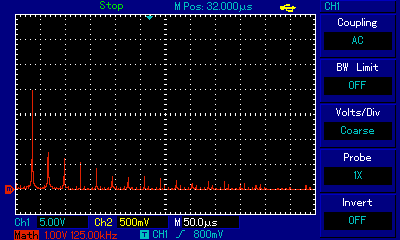
\includegraphics[height=6cm]{picture/SaegeB.PNG}
  \caption{Messwerte für $U_\text{exp, n}$ der Sägezahnspannung.}
  \label{fig:SägeB}
\end{figure}

\begin{table}[H] %Rechteckspannung
  \centering
  \begin{tabular}{c | c | c | c | c |c}
    \toprule
    Oberwelle & $U_\text{exp, n}$ / V & $U_\text{theo, n}$ / V & $\frac{U_\text{exp, n}}{U_1}$ & $\frac{U_\text{theo, n}}{U_1}$ & $\sigma_\text{n}$ \\
    \midrule
    1  & 8.00 & 8.00 & 1.00 & 1.00 & 0.00 \\
    3  & 2.20 & 2.67 & 0.28 & 0.33 & 17.60\\
    5  & 1.60 & 1.60 & 0.20 & 0.20 & 0.00 \\
    7  & 1.00 & 1.14 & 0.13 & 0.14 & 12.28\\
    9  & 1.00 & 0.89 & 0.13 & 0.11 & 12.36\\
    11 & 0.60 & 0.73 & 0.08 & 0.09 & 17.81\\
    \bottomrule
  \end{tabular}
  \caption{Messwerte der Rechteckspannung.}
  \label{tab:Recht}
\end{table}

\begin{figure}[H]
  \centering
  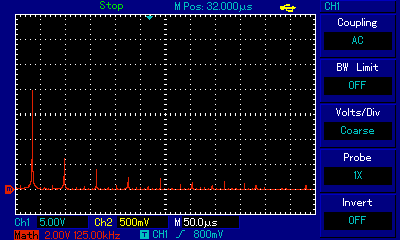
\includegraphics[height=6cm]{picture/RechteckB.PNG}
  \caption{Messwerte für $U_\text{exp, n}$ der Rechteckspannung.}
\end{figure}

\begin{table}[H] %Dreieckspannung
  \centering
  \begin{tabular}{c | c | c | c | c | c}
    \toprule
    Oberwelle & $U_\text{exp, n}$ / V & $U_\text{theo, n}$ / V & $\frac{U_\text{exp, n}}{U_1}$ & $\frac{U_\text{theo, n}}{U_1}$ & $\sigma_\text{n}$ \\
    \midrule
    1  & 5.60 & 5.60 & 1.000 & 1.000 & 0.00 \\
    3  & 0.56 & 0.62 & 0.100 & 0.111 & 9.68 \\
    5  & 0.20 & 0.22 & 0.036 & 0.039 & 9.09 \\
    7  & 0.08 & 0.11 & 0.014 & 0.019 & 27.27\\
    9  & 0.06 & 0.07 & 0.011 & 0.013 & 14.29\\
    11 & 0.03 & 0.05 & 0.005 & 0.009 & 40.00\\
    \bottomrule
  \end{tabular}
  \caption{Messwerte der Dreieckspannung.}
  \label{tab:Drei}
\end{table}

\begin{figure}[H]
  \centering
  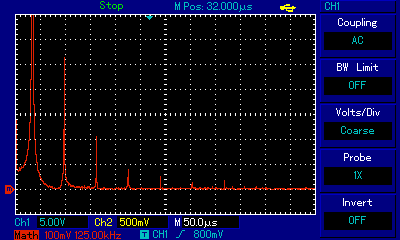
\includegraphics[height=6cm]{picture/DreieckB.PNG}
  \caption{Messwerte für $U_\text{exp, n}$ der Dreieckspannung.}
  \label{fig:DreieckB}
\end{figure}

\newpage
\subsection{Fourier-Synthese}
\label{sec:Synthese}
Die eingestellten Amplituden der Rechteck- und der Sägezahnspannung sind in Tabelle \ref{tab:SagRecht} aufgelistet.

\begin{table}[H]
  \centering
  \begin{tabular}{c c c}
    \toprule
    \multicolumn{2}{c}{Oberwelle} & A / V \\
    Sägezahn & Rechteck & \\
    \midrule
    1. & 1. & 0.640 \\
    2. & --- & 0.320 \\
    3. & 3. & 0.213 \\
    4. & --- & 0.160 \\
    5. & 5. & 0.128 \\
    6. & --- & 0.106 \\
    7. & 7. & 0.091 \\
    8. & --- & 0.080 \\
    9. & 9. & 0.071 \\
    10. & --- & 0.064 \\
    \bottomrule
  \end{tabular}
  \caption{Die eingestellten größen für die Rechteck- und die Sägezahnspannung.}
  \label{tab:SagRecht}
\end{table}

\textbf{Sägezahn-Schwingung:} \\
\begin{figure}[H]
  \centering
  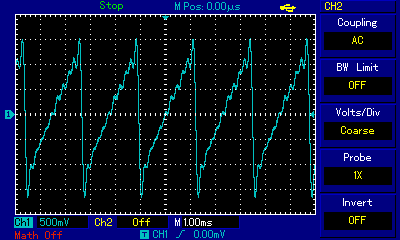
\includegraphics[height=5cm]{picture/Saege.PNG}
  \caption{Sägezahn-Schwingung.}
  \label{fig:Säge}
\end{figure}

\newpage
\textbf{Rechteck-Schwingung:} \\
\begin{figure}[H]
  \centering
  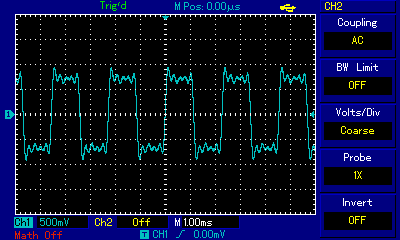
\includegraphics[height=5cm]{picture/Rechteck.PNG}
  \caption{Rechteck-Schwingung.}
  \label{fig:Recht}
\end{figure}

Die eingestellten Amplituden der Rechteck- und der Sägezahnspannung sind in Tabelle \ref{tab:Dreis} aufgelistet.

\begin{table}[H]
  \centering
  \begin{tabular}{c c}
    \toprule
    Oberwelle & A / V \\
    Dreieck & \\
    \midrule
    1. & 0.640 \\
    3. & 0.071 \\
    5. & 0.026 \\
    7. & 0.013 \\
    9. & 0.007 \\
    \bottomrule
  \end{tabular}
  \caption{Die eingestellten größen für die Dreiecksspannung.}
  \label{tab:Dreis}
\end{table}

\textbf{Dreieck-Schwingung:} \\
\begin{figure}[H]
  \centering
  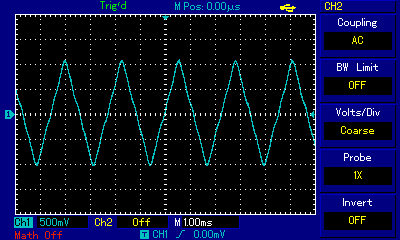
\includegraphics[height=5cm]{picture/Dreieck.PNG}
  \caption{Dreieck-Schwingung.}
  \label{fig:Drei}
\end{figure}
